\documentclass[11pt]{article}
\usepackage[margin=1in]{geometry}
\usepackage[utf8]{inputenc}
\usepackage[T1]{fontenc}
\usepackage{lmodern}
\usepackage{amsmath,amssymb}
\usepackage{graphicx}
\usepackage{booktabs}
\usepackage{xcolor}
\usepackage{listings}
\usepackage{tikz}
\usetikzlibrary{arrows.meta,positioning,fit}
\usepackage[hidelinks]{hyperref}
\usepackage{url}
\usepackage{caption}
\captionsetup{font=small,labelfont=bf}

\newcommand{\memprint}{MemPrint}
\newcommand{\libmpr}{\texttt{libmpr}}
\newcommand{\pass}{\texttt{MemPrintResize}}
\newcommand{\secref}[1]{Section~\ref{#1}}
\newcommand{\figref}[1]{Figure~\ref{#1}}
\newcommand{\tabref}[1]{Table~\ref{#1}}
\newcommand{\term}[1]{\emph{#1}}
\definecolor{mpblue}{HTML}{2a78d6}
\definecolor{mpgrey}{HTML}{52514e}
\lstset{basicstyle=\ttfamily\footnotesize,columns=fullflexible,keepspaces=true,frame=none,
        xleftmargin=1em,showstringspaces=false}

\title{Allocating What Programs Touch:\\
Non-Binding Per-Site Reservations from Measured Memory Footprints}
\author{Nafis Mustakin\\University of California, Riverside}
\date{October 2026}

\begin{document}
\setlength{\emergencystretch}{3em}
\maketitle

\begin{abstract}
A program asks the allocator for the memory it might need, and the operating system and a cluster scheduler
must honour every request, although the program often touches only part of it. We use \memprint{}, a Pin-based
footprint profiler, to measure the bytes each allocation site requests and the bytes the program touches in
each block, and we pass these measurements to the compiler and the runtime as \term{non-binding
reservations}. The system has three parts. First, a per-site mode of the Pin tool records each large block's
touched bytes, highest touched offset and touched pages when the block is freed. Second, \pass{}, an LLVM 21
pass plugin, routes every allocation call through a runtime with a stable site identifier computed from the
call's inlined debug location chain, passes \texttt{std::vector}'s growth capacity through the runtime, and can
embed the reservations in the binary. Third, \libmpr{}, a runtime that is either linked or preloaded, commits only
a block's predicted prefix and maps the rest \texttt{MAP\_NORESERVE}, so that an under-prediction costs commit
accounting and never correctness. \libmpr{} also skips the zeroing of pages that a program has never touched and
keeps those pages out of transparent huge pages. Every program we ran produced its original output under
\libmpr{}. On darknet AlexNet inference, \libmpr{} reduces peak commit by 46.8\%. On miniVite, the pass's
predicted vector capacity reduces peak RSS by 11.5\% and peak commit by 22.5\%. On llama.cpp, which zeroes a KV
cache sized for an 8192-token context, \libmpr{} reduces peak RSS by 49.1\% and peak commit by 34.5\% with a
135M-parameter model (43.3\% and 25.1\% with a 360M model), at no cost in run time, and reservations profiled on
other inputs do as well. Across a 23-program HPC and interpreter corpus, where most programs already hold about
what they touch, \libmpr{} changes no output, keeps run time within $-9\%$ to $+6\%$, and reduces total peak commit
by 10.2\%. We also report what the measurements show about footprint estimation itself: a footprint curve
drawn on wall-clock time needs 24\% less headroom to cover the resident set than one drawn on memory
references, and bytes touched can exceed the resident set when a program writes zeros to fresh memory.
\end{abstract}

\section{Introduction}
\label{sec:intro}

A program's memory request and its memory use are different quantities, and every layer below the program
plans for the request. The allocator maps what is requested, the kernel charges the mapping to the commit
limit~\cite{LinuxOvercommit}, and a batch scheduler on a cluster with disaggregated memory reserves the
request, or an estimate of it, before it places the job~\cite{Zacarias2021Accurate,Li2023Pond}. Our earlier
work built \memprint{}, a Pin-based profiler~\cite{Luk2005Pin,memprint} that measures the bytes a program
touches over its run, and showed that a scheduler which knows a job's footprint curve rather than its request
can pack jobs much more tightly~\cite{memprintsched}. However, a scheduler that reserves less than a program
requests does not change what the program asks for. The program still allocates the full request, and the
kernel still charges it.

The gap between request and use is large in some programs. darknet~\cite{darknet} running AlexNet inference
commits 534.7\,MB and touches 270\,MB, because it allocates training-only weight-update buffers that inference
never uses. llama.cpp~\cite{llamacpp} sizes its KV cache for the model's full 8192-token context and then writes
zeros over all of it, so a 32-token completion holds 189\,MB of cache in RAM and uses 0.4\% of it. miniVite's
edge list grows by doubling, so for a moment the old and new buffers are both live~\cite{minivite}.

Therefore, we ask whether a measured footprint can be passed down to the allocator, so that the program
obtains what it touches rather than what it requests, without trusting the measurement for correctness.
Specifically, we treat \memprint{}'s per-site measurements as \term{non-binding reservations}. A block always
receives every byte the program requested, but only the predicted part is committed, and the rest is mapped so
that the kernel backs it only if the program touches it. A wrong prediction then costs accounting and never
causes a fault the program can observe.

In this work, we make the following contributions:
\begin{itemize}
  \item We extend \memprint{}'s Pin tool to profile requested against touched bytes per allocation site, with
  each block's touched bytes, highest touched offset and touched pages measured exactly when the block is
  freed (\secref{sec:profile}).
  \item We present \pass{}, an LLVM pass plugin that gives every allocation call a stable site identifier from
  its inlined debug location chain, routes it through a runtime, passes \texttt{std::vector}'s new capacity
  through the runtime, and embeds the reservations in the binary (\secref{sec:pass}).
  \item We present \libmpr{}, a runtime that serves large blocks as a committed predicted prefix plus a
  \texttt{MAP\_NORESERVE} remainder, grows blocks by moving page tables, and skips the zeroing of pages that
  were never touched (\secref{sec:runtime}).
  \item We evaluate the system on darknet, miniVite, two LLM inference engines and a 23-program corpus, and we
  show that it halves llama.cpp's resident memory and nearly halves darknet's commit, with identical outputs
  and no time cost (\secref{sec:eval}).
  \item We report what the measurements show about footprint estimation: where miniVite's extra memory comes
  from, why the bytes a program touches can exceed its resident set, and why the time axis of a footprint
  curve matters more than its unit (\secref{sec:discussion}).
\end{itemize}

\section{Background}
\label{sec:background}

\subsection{Three measures of a program's memory}

We use three measures throughout, and the results depend on which one is meant.

\textbf{Bytes touched.} \memprint{}'s footprint is the number of distinct bytes the program has read or
written in memory that is still live, measured from every memory reference under Pin~\cite{memprint}. With
\texttt{-track\_frees}, a freed range leaves the footprint. Bytes touched are a property of the program and its
input, and they do not depend on the allocator or on the page size.

\textbf{Resident set (RSS).} The kernel counts the pages of a process that are in RAM. RSS includes file-backed
pages, such as a memory-mapped model file and the code of every shared library, and it counts a transparent
huge page as 2\,MB~\cite{LinuxTHP}. We sample it from \texttt{/proc/<pid>/smaps\_rollup} every 20\,ms and report
the peak sample. RSS is the quantity the kernel reclaims and the out-of-memory killer acts on, and it is the
"RSS truth" of the scheduling study~\cite{memprintsched}.

\textbf{Commit.} Linux charges private writable mappings to the commit limit when they are
created~\cite{LinuxOvercommit}. We measure commit as the total size of the mappings that
\texttt{/proc/<pid>/smaps} flags \texttt{ac} (accountable), sampled with RSS. A mapping created with
\texttt{MAP\_NORESERVE} is not charged. Under the default heuristic overcommit policy commit is only advisory,
but under strict overcommit (\texttt{vm.overcommit\_memory=2}) it is a hard limit, and in both cases it is the
memory the system has promised to the process.

\subsection{Why untouched memory is often free already}

Linux backs anonymous memory lazily. A large \texttt{malloc} or \texttt{calloc} block is served by \texttt{mmap},
and a page of it becomes resident only when the program first writes it, or reads it, in which case the kernel
maps a shared zero page that RSS does not count. Therefore, a block that the program never touches costs commit
but no RSS. darknet's 250\,MB of unused weight-update buffers are an example. Reducing RSS requires a change in
how memory is obtained, not a smaller reservation. In our measurements RSS fell only where the program, its
allocator, or the kernel touched pages the program did not need: vector growth that keeps two buffers live, a
zeroing \texttt{memset} over fresh memory, and transparent huge pages that back 2\,MB on the first touch.

\subsection{Related work}

Mesh compacts the heap of unmodified C and C++ programs by merging pages whose live objects do not overlap,
and therefore reduces RSS after fragmentation, but unlike our system it does not use a profile of what the
program will touch~\cite{Powers2019Mesh}. Maas et al.\ predict object lifetimes from allocation call stacks to
place long-lived objects together~\cite{Maas2020Llama}, and HALO groups heap objects by profiled access
affinity after link time~\cite{Savage2020HALO}. Both use per-site profiles to change placement, whereas we use
them to change how much of a block is committed and how it is backed. jemalloc and similar allocators return
freed memory to the kernel more eagerly than glibc~\cite{Evans2006jemalloc}, but they still commit every
requested byte. PagedAttention allocates an LLM server's KV cache in blocks as tokens arrive and therefore avoids
reserving a full context per request~\cite{Kwon2023vLLM}. Our llama.cpp result reaches a similar effect for an
unmodified engine, without changing its code, because the untouched part of the cache is never backed.
Zacarias et al.\ show that a 60\% overestimate of memory demand reduces the throughput of a disaggregated
system by about 25\%~\cite{Zacarias2021Accurate}, which is the scheduling motivation for both this work and
our earlier study~\cite{memprintsched}.

\section{Overview}
\label{sec:overview}

\begin{figure}[t]
\centering
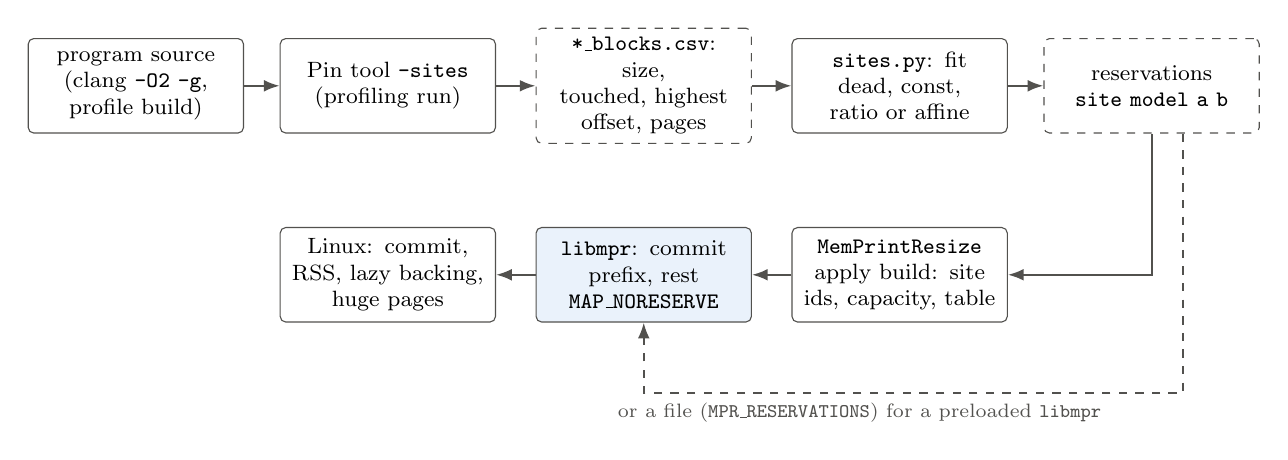
\begin{tikzpicture}[every node/.style={font=\footnotesize},
  box/.style={draw=mpgrey, rounded corners=2pt, align=center, minimum height=12mm, text width=25mm, fill=white},
  data/.style={box, dashed},
  arr/.style={-{Latex[length=2mm]}, mpgrey, thick}]
  \node[box] (src) at (0,0) {program source\\(clang \texttt{-O2 -g},\\profile build)};
  \node[box] (prof) at (3.2,0) {Pin tool \texttt{-sites}\\(profiling run)};
  \node[data] (csv) at (6.45,0) {\texttt{*\_blocks.csv}: size,\\touched, highest\\offset, pages};
  \node[box] (fit) at (9.7,0) {\texttt{sites.py}: fit\\dead, const,\\ratio or affine};
  \node[data] (res) at (12.9,0) {reservations\\\texttt{site model a b}};
  \node[box] (pass) at (9.7,-2.4) {\pass{}\\apply build: site\\ids, capacity, table};
  \node[box, fill=mpblue!10] (rt) at (6.45,-2.4) {\libmpr{}: commit\\prefix, rest\\\texttt{MAP\_NORESERVE}};
  \node[box] (kern) at (3.2,-2.4) {Linux: commit,\\RSS, lazy backing,\\huge pages};
  \draw[arr] (src) -- (prof);
  \draw[arr] (prof) -- (csv);
  \draw[arr] (csv) -- (fit);
  \draw[arr] (fit) -- (res);
  \draw[arr] (res.south) |- (pass.east);
  \draw[arr] (pass) -- (rt);
  \draw[arr] (rt) -- (kern);
  \draw[arr, dashed] ([xshift=4mm]res.south) |- node[below, pos=0.8, font=\scriptsize]{or a file (\texttt{MPR\_RESERVATIONS}) for a preloaded \libmpr{}} (6.45,-3.9) -- (rt.south);
\end{tikzpicture}
\caption{The pipeline. A profiling run of the program under \memprint{}'s Pin tool measures each large block;
\texttt{sites.py} fits one reservation per allocation site; the reservations reach \libmpr{} either embedded in a
binary built with \pass{} or from a file when \libmpr{} is preloaded into an unmodified binary.}
\label{fig:overview}
\end{figure}

\figref{fig:overview} shows the pipeline. First, the program runs once under \memprint{}'s Pin tool with
\texttt{-sites}, which writes one row per large block. Second, \texttt{sites.py} fits each site's reservation
from one or more such runs. Third, the reservations reach \libmpr{}. A program can use the system in two ways.
In the \term{preloaded} configuration, \libmpr{} is loaded with \texttt{LD\_PRELOAD} into an unmodified binary,
a site is the return address of the allocation call, and the reservations come from a file. In the
\term{pass} configuration, the program is built with \pass{}, a site is a hash the compiler computes, and the
reservations can be embedded in the binary. Only the pass configuration can change a vector's growth capacity,
because the capacity is computed inside inlined library code, before any allocation call.

\section{Per-site profiling in \memprint{}}
\label{sec:profile}

The \texttt{-sites} mode of the Pin tool runs with the exact splitter, \texttt{-track\_frees} and the
bytes-touched footprint, which keeps one bit per byte for every touched page. It adds four mechanisms.

\textbf{Site identity.} The tool hooks the allocator's entry points (\texttt{malloc}, \texttt{calloc},
\texttt{realloc}, the aligned variants and every \texttt{operator new}). For the outermost allocator call of a
thread it records the call's return address, written as the image name plus the address in the image file
(for example \texttt{llama-completion+0x92266f}), which stays the same across runs despite address-space
layout randomisation. Because \texttt{operator new} is hooked as an allocator, an allocation made by inlined
standard-library code resolves to the program's own code. In a program built with \pass{}, the tool also hooks
\texttt{\_\_mpr\_alloc} and the other runtime entry points, reads the site identifier from the argument the pass
added, and names the site \texttt{id:0x...}.

\textbf{Block summaries at release.} When a release (a \texttt{free}, a \texttt{realloc} that moves, or an
\texttt{munmap}) is applied, the tool is about to clear the block's bits from the footprint. Just before it does,
it reads the block's touched bytes, the offset of its highest touched byte and its number of touched pages from
the per-page bitmaps. Releases are queued in order with each thread's buffered references, so a summary sees
every reference the program made to the block before freeing it. Blocks still live at exit are summarised at
exit.

\textbf{Allocator zeroing.} \texttt{calloc} served from reused heap memory zeroes the block with a
\texttt{memset} that is not the program's own use. The tool queues a probe at the \texttt{calloc} exit, in order
with the references, and records the bytes touched at that point separately as \texttt{alloc\_touched}.

\textbf{Outputs.} \texttt{*\_blocks.csv} has one row per block of at least 64\,KB with its site, kind, size,
birth and death times, touched bytes, highest touched offset, touched and total pages, allocator-touched
bytes, and whether it was grown from another block. \texttt{*\_sites.csv} aggregates every block per site.
The test suite checks exact values on programs written for the purpose: a dead block, a block touched only in
a prefix, a block touched only at its tail (whose highest touched offset is its size), a \texttt{calloc} on a
reused chunk, a \texttt{realloc} growth chain and a growing vector.

\textbf{Two further options.} In the course of this work we added \texttt{-clock seconds}, under which the
timeline's snapshots are taken every $N$ milliseconds of wall time and every row carries a \texttt{Seconds}
column, and \texttt{-footprint pages}, which counts the 4\,KB pages that hold a touched byte. We use both in
\secref{sec:clock}.

\section{Fitting reservations}
\label{sec:fit}

\texttt{sites.py} reads the blocks of one or more profiling runs, keeps the blocks of at least 64\,KB (the ones
\libmpr{} serves), and fits, per site, the number of bytes a block will need as a function of its requested
size $n$. It fits the highest touched offset rather than the touched bytes, because \libmpr{} commits a block from
its start, so a prediction is safe for a block only if it reaches the block's last touched byte. Four models
are considered:
\begin{itemize}
  \item \texttt{dead}: $0$, when no block of the site was touched;
  \item \texttt{const}: $a$, when the highest offset does not grow with the request;
  \item \texttt{ratio}: $a\,n$;
  \item \texttt{affine}: $a\,n + b$, the lowest line through two blocks that lies above the covered blocks.
\end{itemize}
A model \term{covers} a set of blocks if its prediction reaches each block's highest offset. Among the models
that cover blocks holding at least a quantile $q$ of the site's requested bytes ($q = 0.9$ by default), the fit
keeps the one that commits the least over the training blocks. A site is left out when its best model would
commit at least 95\% of what was requested. The output is one line per site, \texttt{site model a b}, which
\libmpr{} reads at start-up.

A profile can come from the same input the program will run on (we call this \term{own profile}, which
measures the mechanism) or from other inputs of the same program (\term{held out}, which measures how a
reservation transfers). The quantile leaves some blocks uncovered by design, and \secref{sec:robust} shows that
under-predictions are safe.

\section{The \pass{} compiler pass}
\label{sec:pass}

\pass{} is a new-pass-manager plugin for LLVM 21~\cite{Lattner2004LLVM}, 259 lines of C++, loaded into clang with
\texttt{-fpass-plugin}. It registers the same module pass at two extension points of the optimisation pipeline,
and it has three modes: \texttt{profile} (the default) routes allocations through the runtime, \texttt{apply}
also embeds a reservation file, and \texttt{off} does nothing.

\subsection{Allocation calls}

The late instance runs at \texttt{OptimizerLastEP}, after inlining. For every call or invoke whose callee is one
of the allocation functions in \tabref{tab:rules}, it builds a call to the matching runtime entry point with the
original arguments, a site identifier and a kind, replaces every use of the old call, takes over its name and
erases it. \texttt{operator new} under an \texttt{invoke} becomes a plain call followed by a branch to the
invoke's normal destination, because the runtime reports failure the way \texttt{malloc} does, and the
landing pad loses that predecessor. Calls that \texttt{free} memory are not rewritten, because \libmpr{}
recognises its own blocks in \texttt{free}.

\begin{table}[t]
\centering\small
\begin{tabular}{lll}
\toprule
Callee & Runtime entry point & Kind \\
\midrule
\texttt{malloc} & \texttt{\_\_mpr\_alloc(n, site, kind, 0)} & malloc \\
\texttt{calloc} & \texttt{\_\_mpr\_calloc(count, n, site)} & calloc \\
\texttt{realloc} & \texttt{\_\_mpr\_realloc(p, n, site)} & realloc \\
\texttt{aligned\_alloc}, \texttt{memalign}, \texttt{valloc} & \texttt{\_\_mpr\_alloc(n, site, kind, align)} & memalign \\
\texttt{posix\_memalign} & \texttt{\_\_mpr\_posix\_memalign(out, align, n, site)} & memalign \\
\texttt{operator new}, \texttt{new[]}, aligned & \texttt{\_\_mpr\_alloc(n, site, kind, align)} & new \\
\texttt{operator new} (nothrow) & \texttt{\_\_mpr\_alloc(n, site, kind, 0)} & malloc \\
\midrule
result of \texttt{vector<T>::\_M\_check\_len} & \texttt{\_\_mpr\_capacity(len, 0, 1, site)} & (early pass) \\
\bottomrule
\end{tabular}
\caption{The calls \pass{} rewrites.}
\label{tab:rules}
\end{table}

\subsection{Stable site identifiers}

A site identifier must name the same allocation in a profiling build and an apply build, and it must
distinguish allocations that the optimiser has inlined into different callers. \pass{} computes a 64-bit FNV-1a
hash over the callee's name, the name of the function that contains the call after inlining, and the call's
debug location chain from the innermost location outward through every \texttt{inlinedAt} entry, each as file,
line and column. An allocation inside an inlined \texttt{std::allocator::allocate} therefore resolves to the
program line that grew the container. The enclosing function's mangled name is part of the hash, because
inlined library code has the same location for every element type. Without debug information the hash falls
back to the function's name and the call's position in it, so the build needs \texttt{-g} (line tables are
enough). The pass appends one line per site to a site map (\texttt{0x... malloc main.cpp:777:5 ...}), which
links a profile's sites to source lines. On darknet the pass rewrote 631 calls in 48 files, and the profiling and
apply builds produced identical identifiers.

\subsection{Vector growth capacity}

A \texttt{std::vector} that grows by \texttt{push\_back} or \texttt{emplace\_back} doubles its capacity, copies its
elements, and frees the old buffer. libstdc++ computes the new capacity in
\texttt{\_M\_check\_len}, called from \texttt{\_M\_realloc\_insert} and \texttt{\_M\_default\_append}. After
inlining that call no longer exists, so the early instance of the pass runs at \texttt{PipelineStartEP}, before
inlining, and wraps the integer result of every \texttt{\_M\_check\_len} call:
\begin{lstlisting}
%len = call i64 @_ZNKSt6vectorI...E12_M_check_lenEmPKc(ptr %this, i64 1, ptr @.str)
%cap = call i64 @__mpr_capacity(i64 %len, i64 0, i64 1, i64 <site>)   ; uses of %len now use %cap
\end{lstlisting}
The element size is not known at that point, so the pass passes 1 and the capacity model is expressed in
elements. \libmpr{} returns the larger of \texttt{len} and the site's predicted final size, so the first growth
allocates the final capacity and the copy chain disappears. A wrong prediction cannot break the program,
because the capacity only grows, and an over-large capacity is backed lazily. On miniVite the pass rewrote 73
allocation calls and 17 growth points. The pattern is specific to libstdc++ (GCC 8 headers here), and
\secref{sec:limits} discusses the consequence of naming the site before inlining.

\subsection{Embedding reservations}

In apply mode the late instance reads the reservation file and adds it to the module as a constant string,
\texttt{\_\_mpr\_embedded\_reservations}. Every translation unit carries a copy, so the global has
\texttt{weak\_odr} linkage in a COMDAT group of the same name, and the linker keeps one. (\texttt{weak\_any}
kept 48 copies in darknet's shared library, and \texttt{linkonce\_odr} was discarded as unreferenced.) \libmpr{}
declares the symbol weak and reads it at start-up when \texttt{MPR\_RESERVATIONS} is not set, so an apply build
needs no environment.

\subsection{Toolchain notes}

clang parses \texttt{-mllvm} options before it loads a \texttt{-fpass-plugin}, so the plugin's options are not
yet registered when they are parsed. The pass therefore reads \texttt{MPR\_PASS\_MODE},
\texttt{MPR\_PASS\_RESERVATIONS} and \texttt{MPR\_PASS\_SITEMAP} from the environment, and the same settings remain
available as options under \texttt{opt}. On our machine clang found a newer GCC's headers first, so builds pass
\texttt{--gcc-install-dir} for the system GCC 8, whose libstdc++ the programs run with. A build script
(\texttt{scripts/resize\_build.sh}) builds the plugin and \libmpr{}, sets these variables, and runs the program's own
build command. Two \texttt{opt}-plus-FileCheck tests check the rewriting of allocation calls and of a growth point,
and an end-to-end test builds a small program in both modes.

\section{The \libmpr{} runtime}
\label{sec:runtime}

\libmpr{} is about 760 lines of C. It defines \texttt{malloc}, \texttt{calloc}, \texttt{realloc},
\texttt{reallocarray}, \texttt{free}, the aligned allocators, \texttt{malloc\_usable\_size}, the \texttt{operator new}
variants and \texttt{memset}, so it serves both a preloaded binary and a binary built with \pass{}. A block
smaller than \texttt{MPR\_MIN} (64\,KB) or at a site without a reservation goes to glibc through
\texttt{\_\_libc\_malloc} and its siblings, unchanged.

\subsection{Serving a block}

For a large block at a reserved site, \libmpr{} computes the prediction $p$ from the site's model, rounds the
request $n$ and $p$ up to pages, and creates one anonymous mapping of the full size with \texttt{MAP\_NORESERVE}.
It then maps the first $p$ bytes again with \texttt{MAP\_FIXED} and without \texttt{MAP\_NORESERVE}, which makes the
prefix accountable. The program receives a pointer to all $n$ bytes. If it touches beyond $p$, the kernel backs
the page as for any anonymous memory, with no signal the program could observe. A design that protected the
remainder with \texttt{PROT\_NONE} and grew the block on a fault would also break system calls, because a
\texttt{read()} into a protected page returns \texttt{EFAULT} instead of faulting. A \texttt{dead} site's block is
entirely \texttt{MAP\_NORESERVE}. A large \texttt{calloc} needs no \texttt{memset}, because fresh anonymous pages
are zero. Blocks live in an open-addressing table keyed by address, and \texttt{free} recognises a runtime block
by its page alignment and a table lookup, records its resident bytes with \texttt{mincore} for telemetry, and
unmaps it. The tables are themselves mapped \texttt{MAP\_NORESERVE}, so \libmpr{} commits nothing of its own.

\subsection{Growing and shrinking}

A runtime block grows without copying where possible. \libmpr{} first tries to map the new tail directly after
the block with \texttt{MAP\_FIXED\_NOREPLACE}. If the address is taken, it reserves a new range and moves the
block's two mappings into it with \texttt{mremap(MREMAP\_FIXED)}, which moves page tables instead of data.
Growth is geometric, at least 1.5$\times$, so a table grown one element at a time does not remap at every step,
and a shrink is kept in place unless it halves the block. We found two kernel behaviours on the way. The kernel
keeps a tail that was added in place and written separately as its own mapping, and \texttt{mremap} fails with
\texttt{EFAULT} on a range that spans several mappings. A failed \texttt{mremap(MREMAP\_FIXED)} has also already
unmapped its destination. Open MPI's start-up (in \texttt{libpciaccess}) grows a table one element at a time
past the size threshold and crashed on the first version. \libmpr{} now maps the destination again and copies
such a piece.

\subsection{Skipping the zeroing of untouched pages}

Programs that clear a buffer they have just allocated make every page of it resident. \libmpr{} defines
\texttt{memset}. When the value is zero, the range lies in a runtime block, and the block's first page contains
the start of the range, \libmpr{} reads the range's entries from \texttt{/proc/self/pagemap}~\cite{LinuxPagemap}
and writes zeros only to pages that need them:
\begin{itemize}
  \item a page that is neither present (bit 63) nor swapped (bit 62) has never been touched since the block
  was mapped, and it reads as zero, so it is skipped;
  \item a page that is present but not mapped exclusively (bit 56 clear) is the kernel's shared zero page,
  mapped by an earlier read, or a page shared with a forked child, so \libmpr{} reads it and skips it if it
  is all zeros, which is correct in both cases;
  \item every other page, and the partial pages at both ends, are written.
\end{itemize}
Other \texttt{memset} calls go to glibc's implementation, found with \texttt{dlsym(RTLD\_NEXT)} at start-up (a
byte loop that GCC must not turn back into a \texttt{memset} serves the calls made before that).

The first version checked only the present bit. llama.cpp clears its KV cache a second time after a warm-up
decode, and attention had read the whole cache by then, so every page mapped the zero page and looked present.
After the zero-page check, 123\,MB of the cache were still resident. The cause was transparent huge pages,
which this machine enables for all anonymous memory: the warm-up writes a few rows into each layer's K and V
tensors (about 3\,MB each), and each first write faults in a 2\,MB page~\cite{LinuxTHP}. \libmpr{} therefore
marks the pages whose zeroing it skipped \texttt{MADV\_NOHUGEPAGE}. Those are the pages it chose to leave
untouched, and a huge page would undo the choice. Pages the program has touched keep huge pages.
\texttt{MPR\_THP=0} and \texttt{MPR\_THP=1} disable huge pages for all runtime blocks or leave them as the system
sets them, and \texttt{MPR\_ZERO=0} turns the zero skipping off.

\subsection{Telemetry and settings}

With \texttt{MPR\_REPORT}, \libmpr{} writes per site at exit the number of blocks, the bytes requested,
predicted (committed), resident at free, the blocks that used more than predicted, and the zeroing it skipped.
\texttt{\_\_mpr\_committed()} returns the predicted committed total for a scheduler to read.
\texttt{MPR\_SCALE} multiplies every prediction for robustness tests, and \texttt{MPR\_ALL} serves every large block,
reserved or not, to measure the mechanism alone. Two lock-related fixes were needed: \texttt{dladdr}, used to name
a return-address site, is called outside \libmpr{}'s lock, and the exit handler releases the lock before it
writes the report, because \texttt{fclose} frees its buffer through \texttt{free}.

\section{Evaluation}
\label{sec:eval}

\subsection{Setup}

All runs used a two-socket Intel Xeon E5-2620 v4 (16 cores, 32 threads) with 62\,GB of RAM, Linux 4.18 (RHEL 8)
with heuristic overcommit and transparent huge pages set to \texttt{always}, GCC 8.5 and clang 21. Each
configuration ran three times, and we report the mean of the peak RSS and the peak commit, sampled every 20\,ms
for the program and its children. Outputs were compared by hash: all printed lines except those that report a
time or a rate, the modularity line for miniVite, the predictions for darknet, and the generated text for the LLM
engines.

The workloads are:
\begin{itemize}
  \item darknet AlexNet inference on 10 images~\cite{darknet}, built with GCC (preloaded) and with \pass{};
  \item miniVite~\cite{minivite} with 32768 vertices and 4 OpenMP threads, built with GCC and with \pass{};
  \item llama.cpp b11500~\cite{llamacpp}, CPU only, 4 threads, greedy decoding of "Once upon a time" with
  SmolLM2-135M-Instruct (32 and 128 tokens) and SmolLM2-360M-Instruct (64 tokens), both quantised to
  Q8\_0~\cite{SmolLM2}, at the model's default 8192-token context;
  \item llama2.c~\cite{llama2c}, greedy, 128 steps, with the stories15M, 42M and 110M models;
  \item the 23 programs of the scheduling corpus~\cite{memprintsched} at their largest inputs: PolyBench kernels,
  GAP, HPCCG, LULESH, miniFE, Kripke, Quicksilver, NPB, darknet, miniVite, the Lua, Perl and Python
  interpreters, SQLite and GCC's cc1.
\end{itemize}
For the LLM engines and the corpus, \libmpr{} is preloaded, and each input has an own profile and a held-out
profile from the program's other inputs (for darknet, the reference and Extraction networks).

\subsection{Headline results}

\begin{table}[t]
\centering\small
\begin{tabular}{lrrrrrrc}
\toprule
 & \multicolumn{2}{c}{glibc} & \multicolumn{2}{c}{libmpr, own profile} & \multicolumn{2}{c}{libmpr, held out} & Output \\
\cmidrule(lr){2-3}\cmidrule(lr){4-5}\cmidrule(lr){6-7}
Workload & RSS & Commit & RSS & Commit & RSS & Commit & identical \\
\midrule
darknet AlexNet & 287.3 & 534.7 & 287.7 & 284.6 & 287.8 & 519.1 & yes \\
miniVite 32768 (pass) & 30.3 & 46.2 & 27.0 & 26.5 & 28.6 & 32.2 & yes \\
llama.cpp 135M, 32 tok & 380.0 & 404.5 & 175.1 & 55.6 & 175.2 & 56.6 & yes \\
llama.cpp 135M, 128 tok & 380.1 & 404.5 & 177.4 & 56.4 & 177.5 & 56.2 & yes \\
llama.cpp 360M, 64 tok & 768.2 & 560.5 & 419.0 & 56.3 & 424.4 & 57.4 & yes \\
llama2.c 15M & 67.0 & 6.2 & 67.4 & 4.3 & 67.4 & 3.3 & yes \\
llama2.c 42M & 201.0 & 36.2 & 175.9 & 6.8 & 175.8 & 21.6 & yes \\
llama2.c 110M & 514.6 & 78.2 & 452.5 & 12.1 & 469.6 & 45.8 & yes \\
\bottomrule
\end{tabular}

\caption{Peak RSS and peak commit in MB (mean of 3 runs). miniVite's glibc column is the GCC build; its "own
profile" column is the \pass{} build with the predicted \texttt{edgeList} capacity, and its held-out column is
\libmpr{} preloaded into the GCC build with reservations from the 8192 and 16384 inputs. All other rows are
\libmpr{} preloaded, except that darknet's apply build with embedded reservations gives the same 284.6\,MB.}
\label{tab:headline}
\end{table}

\begin{figure}[t]
\centering
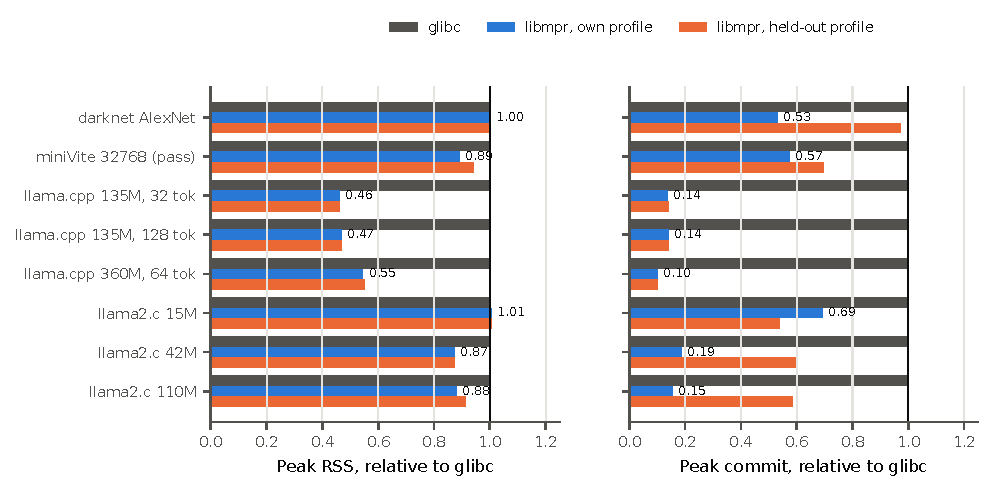
\includegraphics[width=\linewidth]{figures/headline.pdf}
\caption{Peak RSS and peak commit under \libmpr{}, relative to glibc. Every bar is a run whose output was
identical to glibc's.}
\label{fig:headline}
\end{figure}

\tabref{tab:headline} and \figref{fig:headline} summarise the results. \libmpr{} reduces peak commit by 46.8\% on
darknet, by 34.5\% on llama.cpp with the 135M model and by 25.1\% with the 360M model. It reduces peak RSS by
49.1\% and 43.3\% on llama.cpp and by 11.5\% on miniVite through the pass's vector capacity, relative to the pass
build without it. Every run of every workload produced glibc's output, and run time stayed within 5\% of glibc
for every LLM run (darknet 2\%). The two rows where \libmpr{} does little, llama2.c and darknet's held-out
profile, are explained in \secref{sec:llama2c} and \secref{sec:darknet}.

\begin{figure}[t]
\centering
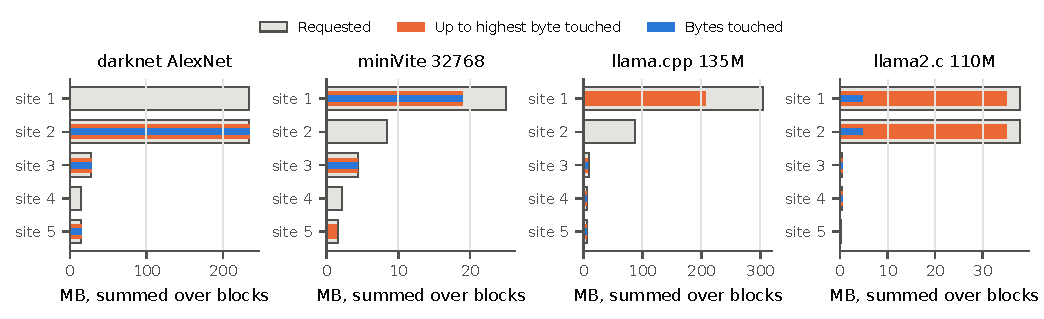
\includegraphics[width=\linewidth]{figures/sites.pdf}
\caption{The five largest allocation sites of four workloads, summed over their blocks: bytes requested, bytes
up to the highest touched offset (what a prefix reservation must commit), and bytes touched. darknet's first
site is dead; llama2.c's two KV caches are touched sparsely across the whole block.}
\label{fig:sites}
\end{figure}

\subsection{darknet: dead training buffers}
\label{sec:darknet}

\figref{fig:sites} shows what the profile found. darknet's largest site allocates the
\texttt{weight\_updates} buffers of its connected layers (\texttt{connected\_\allowbreak layer.c:35}) and convolutional layers
(\texttt{convolutional\_\allowbreak layer.c:196}), which only training uses, so inference never touches them. With its own
profile, \libmpr{} maps them \texttt{MAP\_NORESERVE}, and peak commit falls from 534.7\,MB to 284.6\,MB, close to the
270\,MB the program touches. RSS does not change, because the untouched buffers were never resident. The
\pass{} apply build, with the reservations embedded and no environment, gives the same 284.6\,MB. A held-out
profile from the reference and Extraction networks saves only 15.6\,MB, because those networks have no fully
connected layers: the profile has no data about the connected layers' site, which holds 234\,MB of AlexNet's
untouched buffers, and only the convolutional layers' 15\,MB carry over. A profile helps the code paths it covers.

\subsection{miniVite: vector growth and where its memory goes}
\label{sec:minivite}

\begin{figure}[t]
\centering
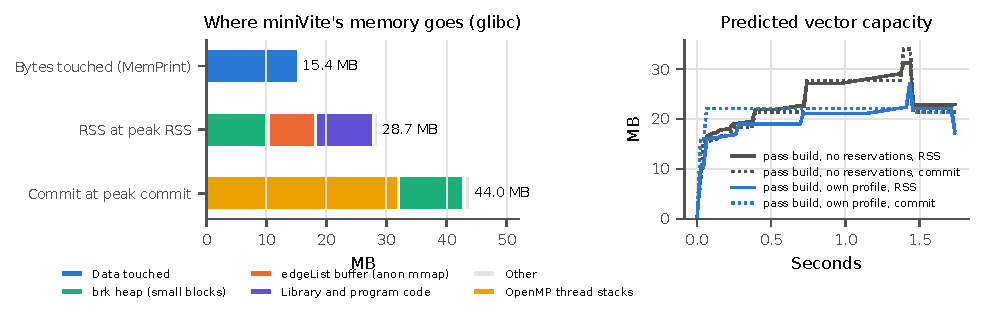
\includegraphics[width=\linewidth]{figures/minivite.pdf}
\caption{Left: miniVite's bytes touched, its RSS at peak RSS and its commit at peak commit under glibc, by
mapping (smaps, 32768 vertices, 4 threads). Right: RSS and commit over time of the \pass{} build without and
with the predicted \texttt{edgeList} capacity.}
\label{fig:minivite}
\end{figure}

miniVite touches 15.4\,MB at its peak but holds 28.7\,MB of RSS at its peak RSS and commits 44.0\,MB at its peak
commit (\figref{fig:minivite}, left). The breakdown, from \texttt{/proc/<pid>/smaps} at each peak, explains the
gap:
\begin{itemize}
  \item \textbf{Code, not data, is a third of the RSS.} 9.6\,MB is library and program code (Open MPI,
  libstdc++, libgomp), which \memprint{} does not count because it measures data references, not instruction
  fetches.
  \item \textbf{Vector growth.} \texttt{edgeList} (\texttt{graph.hpp:777}) grows by \texttt{emplace\_back}
  without \texttt{reserve}, and it is the only large heap site live at the peak. When it doubles, the old
  6.3\,MB buffer and the new 12.6\,MB buffer are both live (18.9\,MB requested, 12.8\,MB touched), and huge pages
  back the new buffer's 6.5 touched MB with about 8\,MB.
  \item \textbf{Small blocks pay glibc's per-chunk overhead.} 1.8 million blocks smaller than 64\,KB (hash table
  nodes of 24 to 47 bytes and small vectors) request 57\,MB over the run but occupy 81\,MB of glibc chunks
  (1.42$\times$), and the heap holds them in 10.4\,MB at the peak.
  \item \textbf{Untouched library memory.} Open MPI's start-up allocates 1.6\,MB that it never touches.
  \item \textbf{Commit is mostly thread stacks.} 32\,MB of the peak commit is four 8\,MB OpenMP thread stacks, of
  which 2\,MB is resident. A smaller \texttt{OMP\_STACKSIZE} would remove that commit, which no allocator change
  can.
\end{itemize}
The growth is what \pass{} can change. The profile of the 32768-vertex input finds that the growth site's final
capacity is 271{,}116 elements (6.5\,MB). With that capacity reserved in the pass build, the vector allocates
once instead of eight times (25\,MB in total), and peak RSS falls from 30.5\,MB to 27.0\,MB and peak commit from
33.6\,MB to 26.1\,MB, with the same modularity and run time (\figref{fig:minivite}, right). Preloaded into the GCC
build with held-out reservations, \libmpr{} reduces RSS from 30.3\,MB to 27.0\,MB through fresh zero pages for the
growth buffers, but it cannot change the capacity.

\subsection{LLM inference}
\label{sec:llm}

\begin{figure}[t]
\centering
\begin{minipage}[b]{0.46\linewidth}
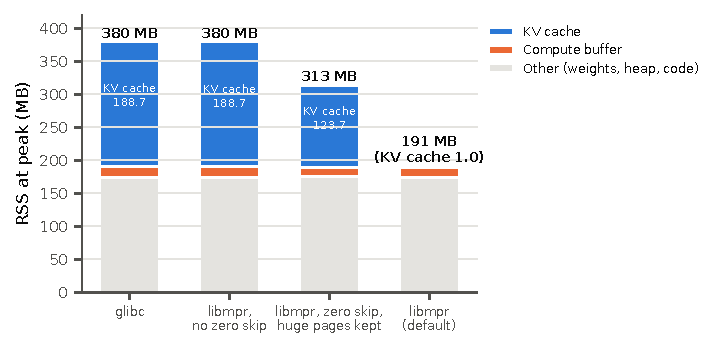
\includegraphics[width=\linewidth]{figures/llamacpp_buffers.pdf}
\end{minipage}\hfill
\begin{minipage}[b]{0.52\linewidth}
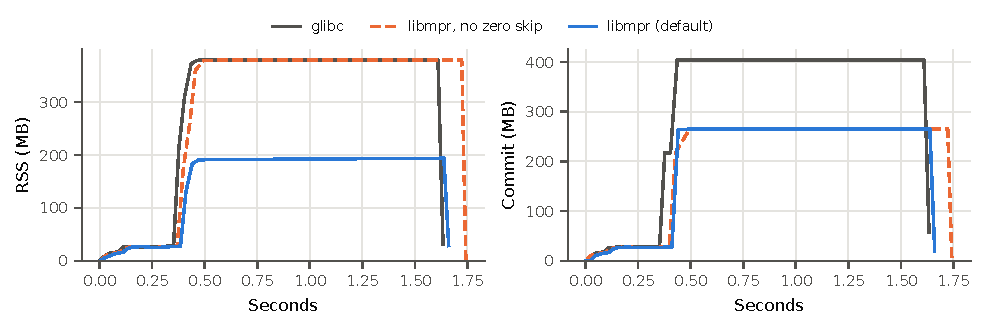
\includegraphics[width=\linewidth]{figures/llamacpp_timeline.pdf}
\end{minipage}
\caption{llama.cpp with SmolLM2-135M. Left: RSS at the peak by buffer, measured from
\texttt{/proc/<pid>/pagemap} over each buffer's address range (32 tokens; "other" is the mapped weights, the
heap and code). Right: RSS and commit over a 128-token run.}
\label{fig:llamacpp}
\end{figure}

\textbf{llama.cpp.} With the 135M model, llama.cpp allocates three large buffers through
\texttt{ggml\_\allowbreak aligned\_\allowbreak malloc}: a 188.7\,MB KV cache for 8192 tokens, a 115\,MB compute buffer whose highest touched
offset is 20.6\,MB, and two 44\,MB scheduler arrays (\texttt{ggml\_backend\_sched\_new}) that are never touched. It
clears the whole KV cache with \texttt{memset} at start-up and again after its warm-up decode. Under glibc, the
whole cache is therefore resident although a 32-token completion uses 0.4\% of it. The model's weights are
mapped from the GGUF file, so their 143\,MB count in RSS but not in commit.

The two savings have different causes (\figref{fig:llamacpp}). Commit falls from 404.5\,MB to 265.1\,MB because of
the reservations: the scheduler arrays are \texttt{dead} and become \texttt{MAP\_NORESERVE}, and only the compute
buffer's 20.6\,MB prefix is committed. The KV cache stays committed in full, because the profile counted the
zeroing as touching all of it. RSS falls from 379.9\,MB to 193.2\,MB because of the zero skipping. To attribute
it, we recorded each buffer's address and measured its resident pages at the peak from
\texttt{/proc/<pid>/pagemap} under four configurations. Without zero skipping, the KV cache holds 188.7\,MB, as
under glibc. Skipping the zeroing alone leaves 123.7\,MB, all of it huge pages faulted in by the warm-up's writes
of one row per layer. Skipping the zeroing and keeping huge pages off the skipped pages leaves 1.0\,MB. The
compute buffer holds 15 to 17\,MB under every configuration, which is the part llama.cpp uses at the peak, and
the remaining 174\,MB (weights, heap and code) does not change. Held-out profiles from the program's other two
inputs give the same results, because the sites are the same code paths at every model size. Run time does not
change (0.85\,s against 0.83\,s for 32 tokens, 2.04\,s against 2.14\,s for the 360M model).

\label{sec:llama2c}
\textbf{llama2.c.} llama2.c is not darknet-like in the same way. Its KV caches are also sized for the full
sequence (37.7\,MB each for the 110M model, of which 4.7\,MB is touched for 128 of 1024 positions), but it
allocates them with \texttt{calloc} and does not clear them, so their untouched part was never resident. They are
laid out as [layer][position][dimension], so every layer's first rows are touched and the highest touched offset
lies at 93\% of the block (\figref{fig:sites}). A prefix reservation must cover it, and commit falls by only 7\%
(78.2\,MB to 72.8\,MB). Committing only the touched pages would need a reservation shaped like the use, for
example a period and a prefix per period, which we have not built. RSS is dominated by the memory-mapped weights
and does not change.

\subsection{The corpus: no regressions}

\begin{table}[t]
\centering\small
\begin{tabular}{lrrr}
\toprule
23 programs, largest inputs & glibc & libmpr, own & libmpr, held out \\
\midrule
Total peak commit (MB) & 2{,}504 & 2{,}249 & 2{,}487 \\
Total peak RSS (MB) & 2{,}293 & 2{,}285 & 2{,}286 \\
Median commit / touched & 1.01 & 1.01 & 1.01 \\
Median RSS / touched & 1.05 & 1.05 & 1.05 \\
Time relative to glibc (range) & 1 & 0.91 to 1.06 & 0.94 to 1.04 \\
Programs with identical output & -- & 23 of 23 & 23 of 23 \\
\bottomrule
\end{tabular}

\caption{The 23 programs of the scheduling corpus at their largest inputs (3 runs each).}
\label{tab:corpus}
\end{table}

\begin{figure}[t]
\centering
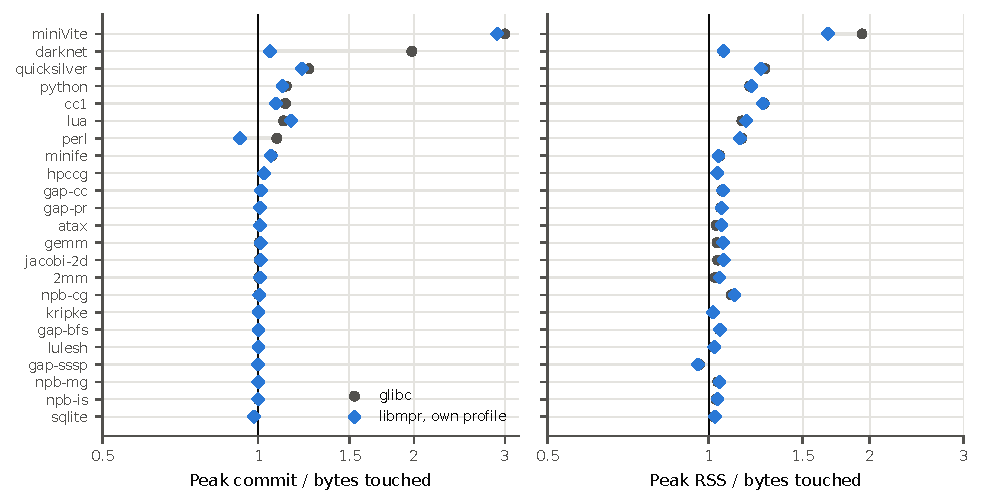
\includegraphics[width=\linewidth]{figures/corpus.pdf}
\caption{Peak commit and peak RSS relative to bytes touched for the 23 corpus programs, under glibc and under
\libmpr{} with each program's own profile. Most programs already sit at about 1.}
\label{fig:corpus}
\end{figure}

\tabref{tab:corpus} and \figref{fig:corpus} show the 23-program corpus. Under glibc, the median program commits
1.01$\times$ its bytes touched and holds 1.05$\times$ in RSS, so there is little for a resizer to take. The
exceptions are darknet (1.98$\times$ commit), miniVite (3.00$\times$), Quicksilver (1.25$\times$), cc1 and Python
(1.13$\times$) and Lua (1.12$\times$). With own profiles, total peak commit falls by 10.2\%, from 2{,}504\,MB to
2{,}249\,MB, nearly all of it darknet's. Held-out profiles save 0.7\%. Lua's commit rises by about 2\,MB, because
its tables grow by \texttt{realloc} and leave the heap for runtime blocks. Every program produced glibc's output in
every run, and run time stayed between 0.91$\times$ and 1.06$\times$ of glibc. The second version of \libmpr{},
with zero skipping and the huge-page policy, changed no program's result relative to the first: total RSS moved
from 2{,}286\,MB to 2{,}285\,MB.

\subsection{Robustness to wrong predictions}
\label{sec:robust}

Under-prediction is safe by construction, and we tested it. With every prediction multiplied by 0.1
(\texttt{MPR\_SCALE=0.1}), darknet and miniVite produced identical outputs, and the telemetry reported the
blocks that used more than predicted. The quantile in the fit leaves blocks uncovered by design, and held-out
profiles under-predict on the LLM engines and the corpus, again with identical outputs. Over-prediction costs
commit and nothing else, because the committed prefix is still backed lazily. Two control programs with no
waste, PolyBench 2mm and HPCCG, with \libmpr{} serving every large block (\texttt{MPR\_ALL}), changed by at most
1.8\,MB of RSS and 0.1\,MB of commit.

\subsection{Effect on scheduling}
\label{sec:schedeffect}

\begin{table}[t]
\centering\small
\begin{tabular}{lrrr}
\toprule
Oracle & Truth: bytes touched & Truth: RSS & Truth: RSS under libmpr \\
\midrule
Exact curve & 90 & 91 & 103 \\
Exact peak & 460 & 436 & 457 \\
MemPrint W5 & 391 & 1{,}807 & 1{,}727 \\
DHAT peak & 979 & 1{,}277 & 1{,}230 \\
User request & 2{,}215 & 2{,}197 & 2{,}204 \\
\bottomrule
\end{tabular}

\caption{Mean response time (minutes) at 80\% offered load in the DMSched-Sim scheduler of our earlier
study~\cite{memprintsched}, with calibrated margins, under three truths of what a job holds. The third truth is
each program's RSS when it runs with \libmpr{} and its own profile.}
\label{tab:sched}
\end{table}

Our earlier study replayed the corpus's measured footprints through a simulator of 32 nodes with a shared
memory pool~\cite{memprintsched}. We added a third truth, the RSS of each program under \libmpr{}
(\tabref{tab:sched}). The results hardly move from the RSS truth, because the corpus programs' resident memory
hardly moved: the exact curve gives 103 minutes (91 under the RSS truth) and MemPrint's windowed curves 1{,}727
(1{,}807). The scheduling study's conclusions therefore do not depend on resizing allocations, since its gain
comes from reserving a curve instead of a peak. Resizing matters for programs that commit or hold much more than
they touch, such as darknet and llama.cpp, and for systems with strict overcommit, where the saved commit is
memory that can be promised to other jobs.

\section{Discussion}
\label{sec:discussion}

\subsection{The time axis of a footprint curve}
\label{sec:clock}

\begin{table}[t]
\centering\small
\begin{tabular}{lrrr}
\toprule
MemPrint curve & Median margin & 90th percentile & Response (min) \\
\midrule
Full trace, bytes, references & 0.06 & 0.58 & 1{,}847 \\
Full trace, bytes, seconds & 0.08 & 0.44 & 1{,}476 \\
Full trace, pages, references & 0.03 & 0.56 & 1{,}942 \\
Full trace, pages, seconds & 0.05 & 0.41 & 1{,}423 \\
W5, bytes, references & 0.04 & 0.58 & 1{,}807 \\
W5, bytes, seconds & 0.04 & 0.56 & 1{,}820 \\
W5, pages, references & 0.04 & 0.58 & 1{,}979 \\
W5, pages, seconds & 0.04 & 0.49 & 1{,}705 \\
\midrule
Exact RSS peak & -- & -- & 436 \\
Exact RSS curve & -- & -- & 91 \\
User request & -- & -- & 2{,}197 \\
\bottomrule
\end{tabular}

\caption{MemPrint's footprint curves under the RSS truth, with the Pin tool's clock and unit options: the margin
(headroom as a share of the curve's peak) each program needs for the curve never to fall below its RSS, over 23
programs, and the mean response time at 80\% load with calibrated margins.}
\label{tab:clock}
\end{table}

\begin{figure}[t]
\centering
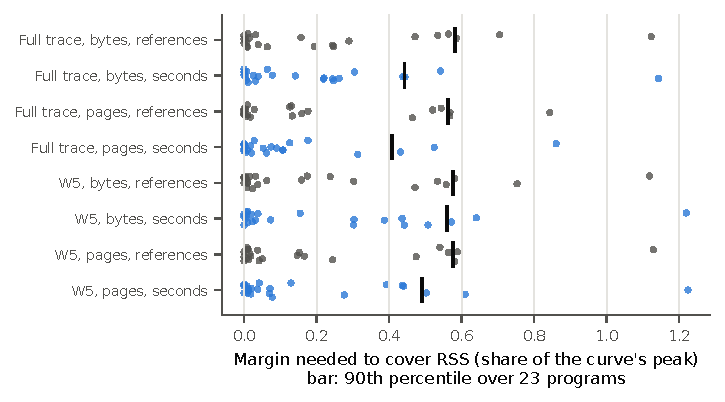
\includegraphics[width=0.7\linewidth]{figures/margins.pdf}
\caption{The margin each corpus program needs (dots; blue: wall-clock axis) and the 90th percentile over
programs (bars), which sets the calibrated margin.}
\label{fig:margins}
\end{figure}

In the scheduling study, a \memprint{} curve needed about 60\% headroom to cover the RSS truth, and we attributed
part of that to the time axis, since \memprint{} counts memory references while RSS is sampled in
seconds~\cite{memprintsched}. The new options let us test the attribution. We reran the full trace and the 5\%
windowed mode at every program's largest input with \texttt{-footprint pages}, and mapped each curve to the wall
time recorded in the \texttt{Seconds} column (\tabref{tab:clock}, \figref{fig:margins}). On wall time, the full
trace's 90th-percentile margin falls from 0.58 to 0.44, and the mean response time from 1{,}847 to 1{,}476
minutes. The programs that gain most have phases that are short in references but long in time, such as GAP BFS
(margin 0.53 to 0.06), GAP CC (0.56 to 0.09) and Lua (0.70 to 0.05). Counting pages instead of bytes helps the
programs whose touched bytes are scattered (cc1 0.25 to 0.13, Perl 0.29 to 0.13, miniVite 1.12 to 0.84), but it
does not reduce the calibrated margin on its own. Together the two options give 0.41 and 1{,}423 minutes, still far
from the exact peak's 436 minutes. The remaining margin comes from memory that \memprint{} does not count, such
as miniVite's library code, which the scheduler's RSS baseline (the run's smallest sample, taken before MPI
loads its libraries) treats as footprint. The wall time is measured under Pin, which slows phases unevenly, so
it approximates native time.

\subsection{Bytes touched can exceed the resident set}

Under \libmpr{}, llama.cpp's RSS (193\,MB) falls below its bytes touched as \memprint{} measures them (353\,MB at
the peak, with the mapped weights). The difference is the zeroing \texttt{memset}: writing zeros to fresh
anonymous memory counts as touching it, although no reader can distinguish the result from untouched memory.
The Pin tool already records \texttt{calloc}'s own zeroing separately. Recording a program's zeroing of
untouched memory in the same way would make the profile, and therefore the reservation, reflect what the
program uses, and it would let \libmpr{} commit less of the KV cache as well.

\subsection{What the RSS numbers measure}

The RSS figures in this paper are peaks of samples of \texttt{smaps\_rollup}, taken every 20\,ms, so a spike
shorter than the interval can be missed. They include file-backed pages and count a huge page as 2\,MB. The
per-buffer figures for llama.cpp come from a different instrument. A logging library recorded where glibc (or
\libmpr{}) placed each buffer of at least 1\,MB, without changing how it allocated, and at the sample with the
largest total RSS we counted each buffer's pages that pagemap reports as present and mapped exclusively, which
excludes the shared zero page. Under glibc the KV cache and the compute buffer lie in one merged mapping, so
\texttt{smaps} alone cannot separate them.

\subsection{Where resizing pays}

The results separate three cases. A program that allocates buffers it never touches (darknet, llama.cpp's
scheduler arrays) gains commit but no RSS, because the kernel never backed those buffers. A program whose
allocator or own code touches memory it does not need (a zeroing \texttt{memset}, vector doubling, huge pages over
sparse writes) gains RSS, and only a change in how the memory is obtained recovers it. A program that already
uses what it allocates, which is the median program in our corpus, gains nothing and loses nothing.

\section{Limitations and future work}
\label{sec:limits}

A limitation of prefix reservations is that a block is committed from its start up to the highest predicted
offset, which commits most of a block that is used sparsely across its whole length, as llama2.c's KV caches
are. A reservation shaped like the use, committing a prefix of each of several periods, would need the Pin tool
to record the touched ranges of each block rather than only its highest offset.

A limitation of the vector capacity is that the early pass names the growth site before inlining, inside
\texttt{\_M\_realloc\_insert<T, Args...>}, so one capacity applies to every vector of that instantiation, and a
capacity measured on one input does not transfer to another, because the final size depends on the input.
Predicting it before the run would need \memprint{}'s static route, which estimates footprints from source and
does not yet produce per-site profiles. The pattern is also specific to libstdc++.

Small blocks are left to glibc, so the per-chunk overhead of small allocations, 1.42$\times$ in miniVite, is not
addressed. Allocators inside interpreters (pymalloc, Lua's tables) and custom \texttt{operator new} are not
covered beyond the large blocks they request from the system.

The commit saving depends on the overcommit policy. Under strict overcommit the kernel ignores
\texttt{MAP\_NORESERVE}, so the saving disappears, although correctness is unaffected. The zero skipping reads
pagemap, which unprivileged processes may read on this kernel without page frame numbers, and its zero-page check
treats a page shared after \texttt{fork} conservatively by reading it.

Profiling is expensive: the Pin tool's exact mode with \texttt{-sites} took 328\,s for a 0.86\,s llama.cpp run and
528\,s for llama2.c 110M (18\,s natively), so profiles must be reused across runs, which the held-out results show
is possible when the inputs exercise the same code paths.

\section{Conclusion}
\label{sec:conclusion}

We passed \memprint{}'s measured per-site footprints to a compiler pass and a runtime as non-binding
reservations, so that a program is backed by what it touches rather than what it requests, and an
under-prediction costs accounting instead of correctness. Every program we ran produced its original output.
\libmpr{} reduced darknet's commit by 46.8\% and halved llama.cpp's resident memory, the pass's predicted vector
capacity removed miniVite's growth chain, and the 23-program corpus, which already holds about what it touches,
saw no regressions. The measurements also showed that a footprint curve is most useful to a scheduler on a
wall-clock axis, and that the bytes a program touches include zeros it writes to fresh memory, which a resident
set does not.

\bibliographystyle{plain}
\bibliography{references}

\end{document}
